\documentclass[xcolor=dvipsnames]{beamer}

\usepackage{amsmath, amssymb, graphicx}
\usepackage[english]{babel}
\usepackage{times}
\usepackage[utf8]{inputenc}
\usepackage[T1]{fontenc}
\usepackage{listings}
\usepackage[norelsize,ruled,vlined]{algorithm2e}
\usepackage{color}
\usepackage{hyperref}
\usepackage{listings}
\usepackage{booktabs}
\usepackage{listings}
\usepackage{tikz}
\usepackage{xcolor}
\usepackage[style=authoryear]{biblatex}
\usepackage{caption}
\usetikzlibrary{matrix}
\usetikzlibrary{arrows}
\usetikzlibrary{positioning}
\usetikzlibrary{shapes.multipart}

\theoremstyle{definition}
\newtheorem{proposition}{Proposition}
\DeclareCaptionFont{white}{\color{white}}
\DeclareCaptionFormat{listing}{\colorbox[cmyk]{0.43, 0.35, 0.35,0.01}{\parbox{\textwidth}{\hspace{15pt}#1#2#3} } }
\captionsetup[lstlisting]{format=listing, labelfont=white, textfont=white, singlelinecheck=false, margin=0pt, font={bf,footnotesize} }
\addbibresource{project.bib}

\newcommand{\fancyh}{\mathcal{H}}
\newcommand{\gangle}[1]{\langle{} #1 \rangle{}}
\newcommand{\myd}{\mathrm{d}}
\newcommand{\NN}{\mathbb{N}}
\newcommand{\RR}{\mathbb{R}}
\newcommand{\ZZ}{\mathbb{Z}}

\definecolor{dkgreen}{rgb}{0,0.6,0}
\definecolor{gray}{rgb}{0.5,0.5,0.5}
\definecolor{mauve}{rgb}{0.58,0,0.82}

\lstset{language=Scala,
  aboveskip=3mm,
  basicstyle={\normalsize\ttfamily},
  belowskip=3mm,
  gobble=20,
  breakatwhitespace=true,
  breaklines=true,
  columns=flexible,
  commentstyle=\color{dkgreen},
  keywordstyle=\color{blue},
  numbers=none,
  numberstyle=\tiny\color{gray},
  showstringspaces=false,
  stepnumber=1,
  keepspaces=true,
  showstringspaces=false,
  stringstyle=\color{mauve},
  tabsize=2,
}

\mode<presentation>
{\setbeamertemplate{navigation symbols}{}
    \setbeamertemplate{items}[ball]
    % \setbeamertemplate{blocks}[rounded][shadow=true]
    \beamertemplatenavigationsymbolsempty
    \usecolortheme[named=Sepia]{structure}
    \usetheme{Warsaw}
    \useoutertheme{infolines}
    \setbeamercovered{transparent}
}

\definecolor{mygreen}{rgb}{0, 178, 115}

\tikzstyle{block} = [rectangle, draw, font=\tiny, text centered, rounded corners, minimum height=1em, node distance=1.5cm, minimum width=2em]
\tikzstyle{line} = [draw, -latex']
\tikzstyle{value} = [label, black, font=\tiny, thick, node distance=0.4cm]

\title[scalafmt]{scalafmt: opinionated \\ code formatter for Scala}
\author{Ólafur Páll Geirsson}
% \department{School of Computer and Communication Sciences}
% \project{Semester Project}
\institute[EPFL]{École Polytechnique Fédérale de Lausanne \\
    School of Computer and Communication Sciences\\
\logoepfl}
\date{\today}

% Delete this, if you do not want the table of contents to pop up at
% the beginning of each subsection:
\AtBeginSection[]
{\begin{frame}<beamer>{Overview}
  \tableofcontents[
    sections={1-6},
            currentsection,
            currentsubsection,
            hideothersubsections,
            sectionstyle=show/shaded,
        subsectionstyle=show/shaded/hide]
\end{frame}
}

\begin{document}

\newcommand{\logoepfl}[0]{\begin{center}
  
\includegraphics[width=2cm]{logo_epfl_coul.eps}
    \vspace{-0.5cm}
\end{center}
}


%%%%%%%%%%%%%%%%%%%%%%%%%%%%%%%%%%%%%%%%%%%%%%%%%%%%%%%%%%%%%%%
% 0. Titlepage
%%%%%%%%%%%%%%%%%%%%%%%%%%%%%%%%%%%%%%%%%%%%%%%%%%%%%%%%%%%%%%%
\begin{frame}
  \titlepage{}
\end{frame}
\begin{frame}{Today's agenda}
  \tableofcontents[
    sections={1-6},
    hideallsubsections
  ]
\end{frame}

%%%%%%%%%%%%%%%%%%%%%%%%%%%%%%%%%%%%%%%%%%%%%%%%%%%%%%%%%%%%%%%
% 1. Introduction
%%%%%%%%%%%%%%%%%%%%%%%%%%%%%%%%%%%%%%%%%%%%%%%%%%%%%%%%%%%%%%%
\section{Introduction} % (fold)
\label{sec:Introduction}

\begin{frame}{What is code formatting?}
  \begin{block}{Unformatted}
    \lstinputlisting[label={lst:unformatted}]{code/unformatted.scala}
  \end{block}
\end{frame}

\begin{frame}{What is code formatting?}
  \begin{block}{Formatted}
    \lstinputlisting[label={lst:unformatted}]{target/formatted1.scala}
  \end{block}
\end{frame}

\begin{frame}{}
  \begin{center}
    \Huge
    Why?
  \end{center}
\end{frame}

\begin{frame}{Reason 1: Collaborative environments}
  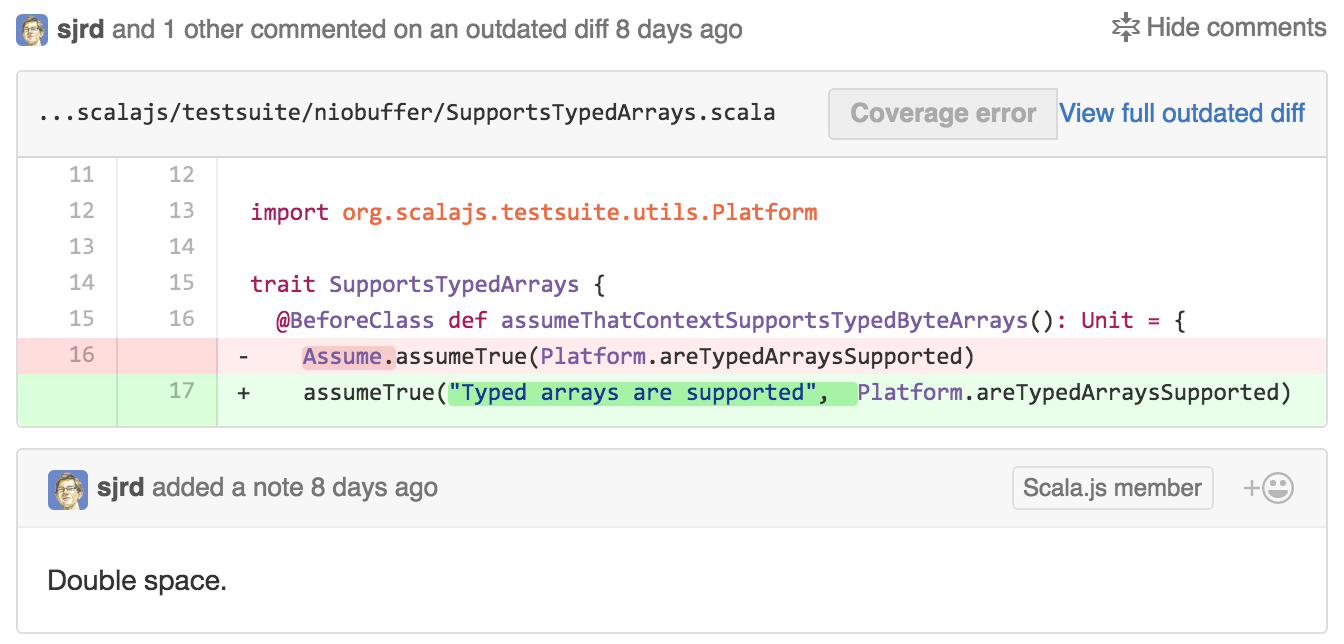
\includegraphics[width=\textwidth]{img/codereview.png}
\end{frame}

\begin{frame}{Reason 2: Refactoring}
  Large-Scale Automated Refactoring Using ClangMR\footnote{Source: http://research.google.com/pubs/pub41342.html}
  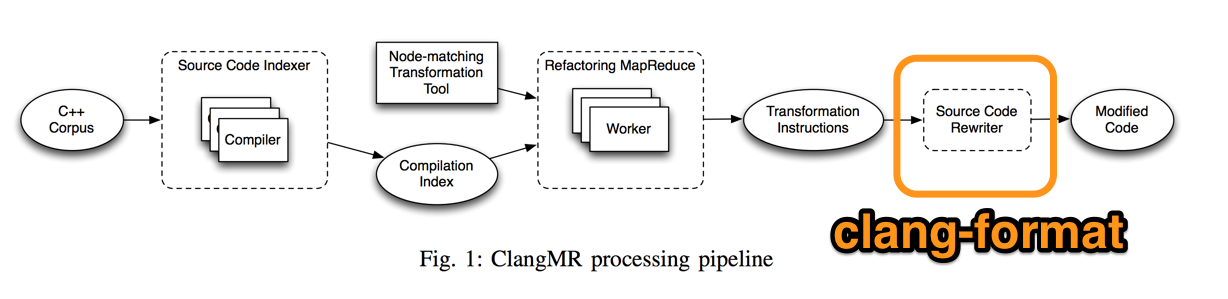
\includegraphics[width=\textwidth]{img/clangmr.png}
\end{frame}

\begin{frame}{Problem statement}
  \begin{block}{}
    What \emph{algorithms} and \emph{data structures} allow us to develop a
    Scala code formatter with the following features?
    \begin{itemize}
      \item \emph{Maximum line length setting}
      \item \emph{Opinionated setting}
      \item \emph{Vertical alignment}
      \item \emph{Good performance}
    \end{itemize}
  \end{block}
\end{frame}

\begin{frame}{Maximum line length setting}
  \lstinputlisting{code/linelength.scala}
\end{frame}

\begin{frame}{Opinionated setting}
  \begin{block}{My definition}
    Disregard line breaking decisions in the original source to ensure that
    formatted sources follow a uniform coding style.
  \end{block}
  \lstinputlisting{code/binpack.scala}
\end{frame}

\begin{frame}{Vertical alignment}
  \lstinputlisting{code/align.scala}
\end{frame}

\begin{frame}{Performance}
  \begin{itemize}
    \item IDEs: reformat file on save
    \item Build tools: reformat file on compile
    \item Continuous integration: reformat diff before code review
  \end{itemize}
\end{frame}

%%%%%%%%%%%%%%%%%%%%%%%%%%%%%%%%%%%%%%%%%%%%%%%%%%%%%%%%%%%%%%%
% 2. Scalafmt
%%%%%%%%%%%%%%%%%%%%%%%%%%%%%%%%%%%%%%%%%%%%%%%%%%%%%%%%%%%%%%%
\section{Background} % (fold)
\label{sec:Background}
\subsection{Scalariform (2010)}

\begin{frame}{Scalariform}
  \begin{itemize}
    \item No maximum line length setting
    \item No opinionated setting
  \end{itemize}
\end{frame}

\subsection{ClangFormat (2013)}

\begin{frame}{}
  \begin{center}
    \Huge ClangFormat\footnote{Source: \url{https://www.youtube.com/watch?v=s7JmdCfI__c}}
  \end{center}
\end{frame}
\begin{frame}{Parser}
  \begin{itemize}
    \item Custom \emph{UnwrappedLine} parser for C, C++, Objective-C, Java,
      JavaScript and Protobuf
      \begin{itemize}
        \item handles invalid code code
        \item $\sim$4.000 LOC
      \end{itemize}
      \begin{center}
        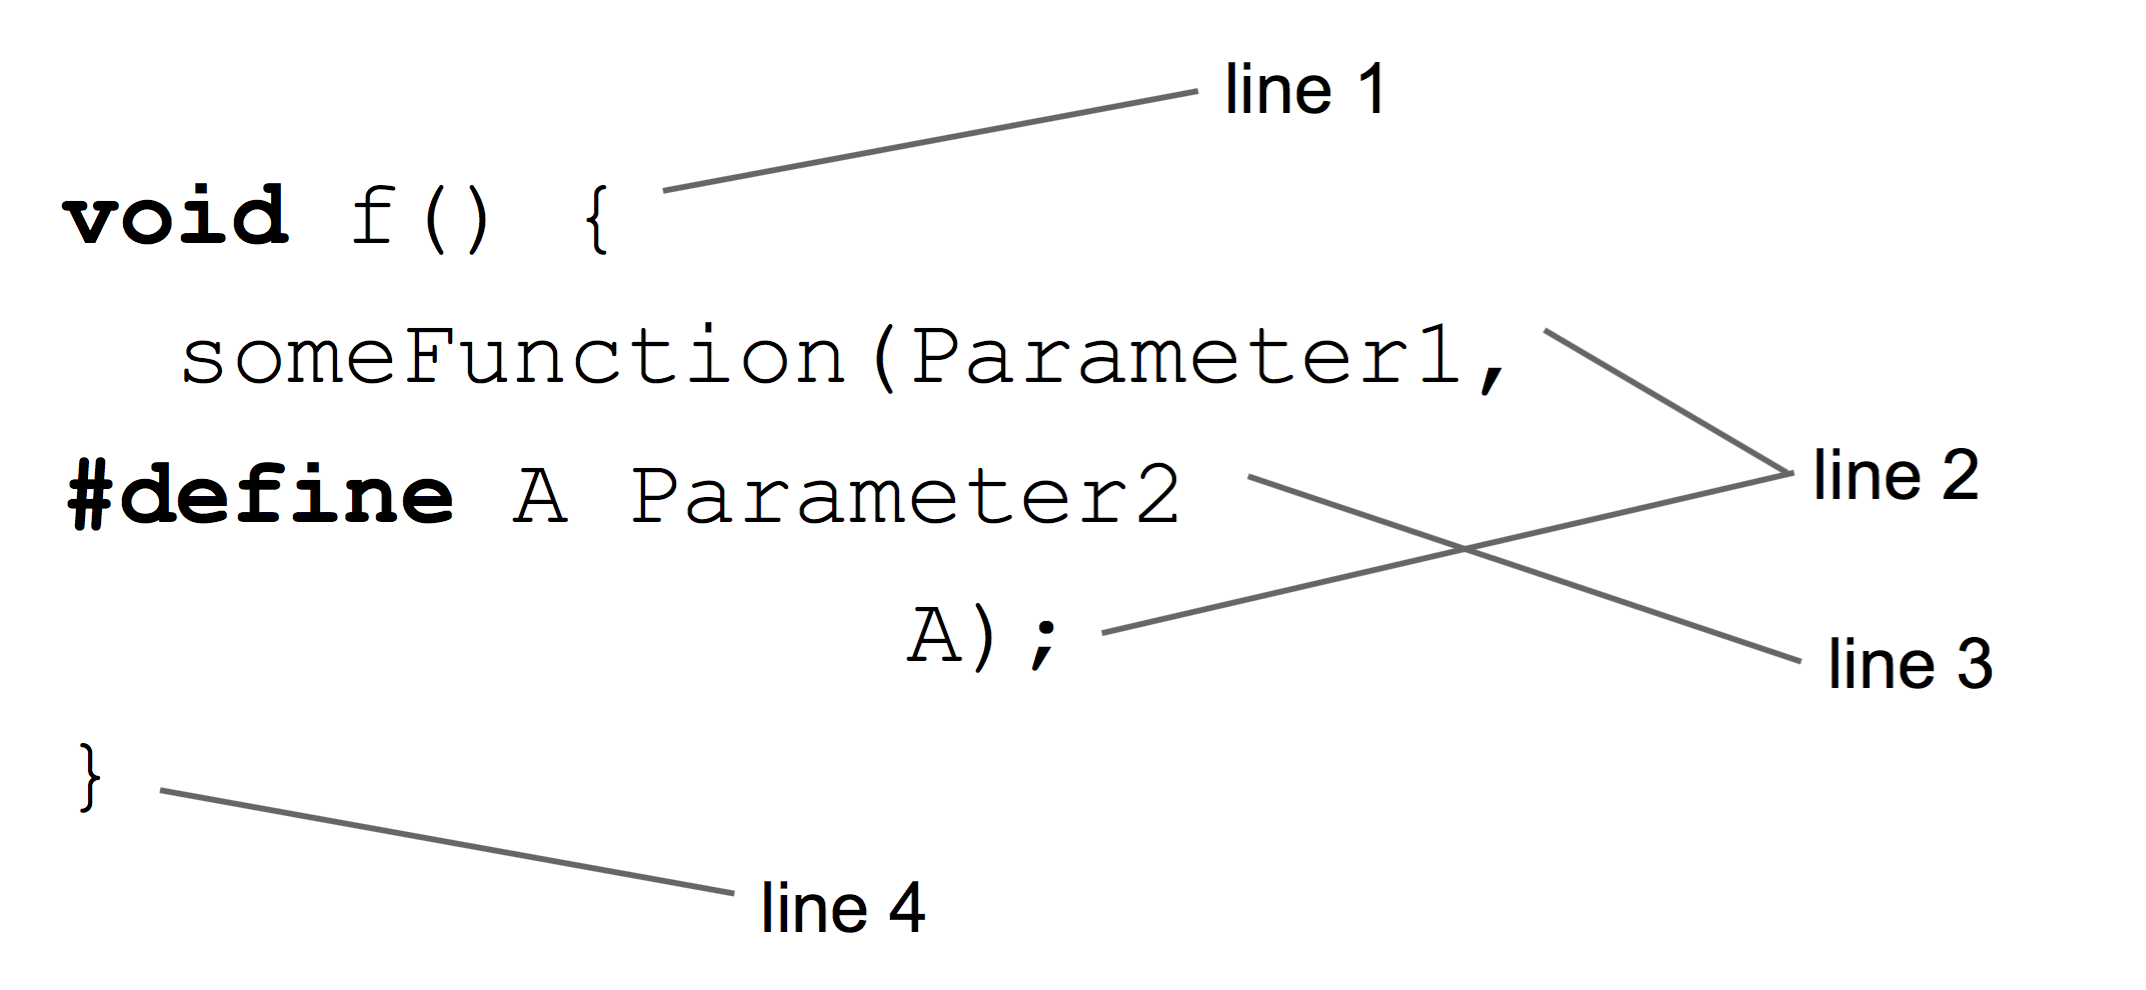
\includegraphics[width=0.8\textwidth]{img/unwrapped.png}
      \end{center}
  \end{itemize}
\end{frame}

\begin{frame}{Line breaking: shortest path search}
  \begin{itemize}
    \item Dijkstra's shortest path for optimal line breaking.
      \begin{itemize}
        \item Non-whitespace tokens are nodes
        \item Whitespace tokens are edges
      \end{itemize}
  \end{itemize}
  \begin{center}
    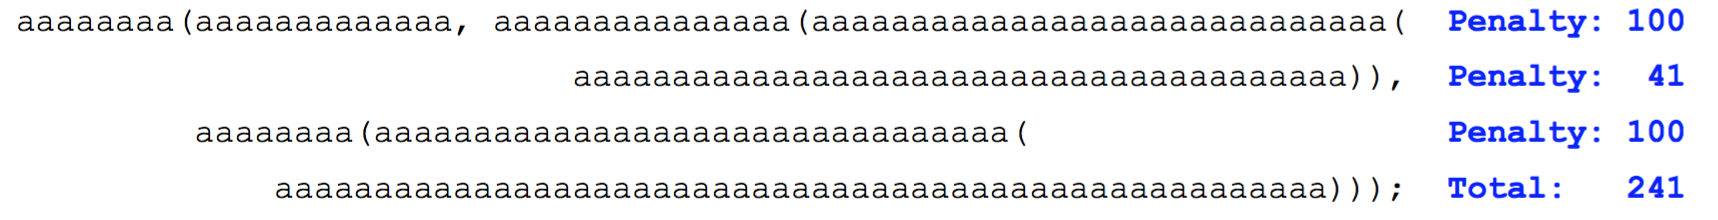
\includegraphics[width=0.8\textwidth]{img/dijkstra.png}
  \end{center}
\end{frame}

\subsection{rfmt (2016)}
\begin{frame}{}
  \begin{center}
    \Huge rfmt\footnote{Source: \url{http://research.google.com/pubs/pub44667.html}}
  \end{center}
\end{frame}

\begin{frame}{Formatting algebra}
  \begin{itemize}
      \item Three layout operators
        \begin{center}
          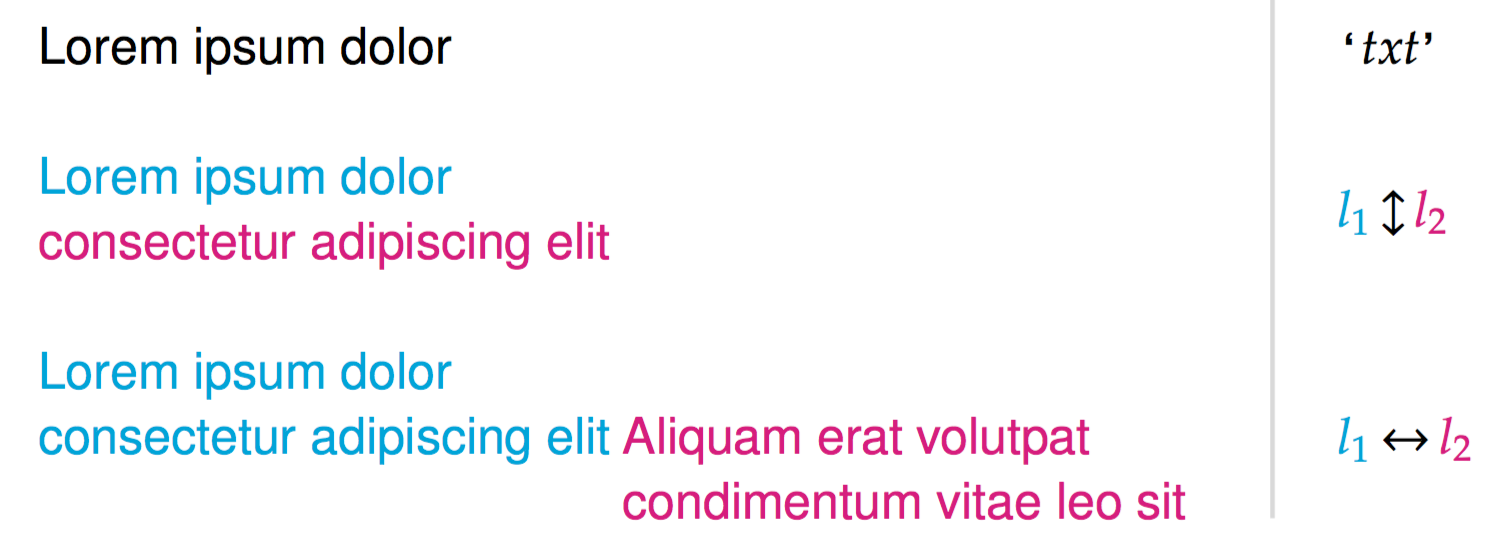
\includegraphics[width=0.8\textwidth]{img/layouts-rfmt.png}
        \end{center}
    \item one \emph{choice} operator ``?''
  \end{itemize}
\end{frame}
\begin{frame}{Translating R to formatting algebra}
  \begin{itemize}
    \item Custom R parser
      \begin{itemize}
        \item $\sim$1.000 LOC
        \item Comments are AST nodes
      \end{itemize}
      \item ``Block language'' implemented in terms of primitive combinators
        \begin{center}
          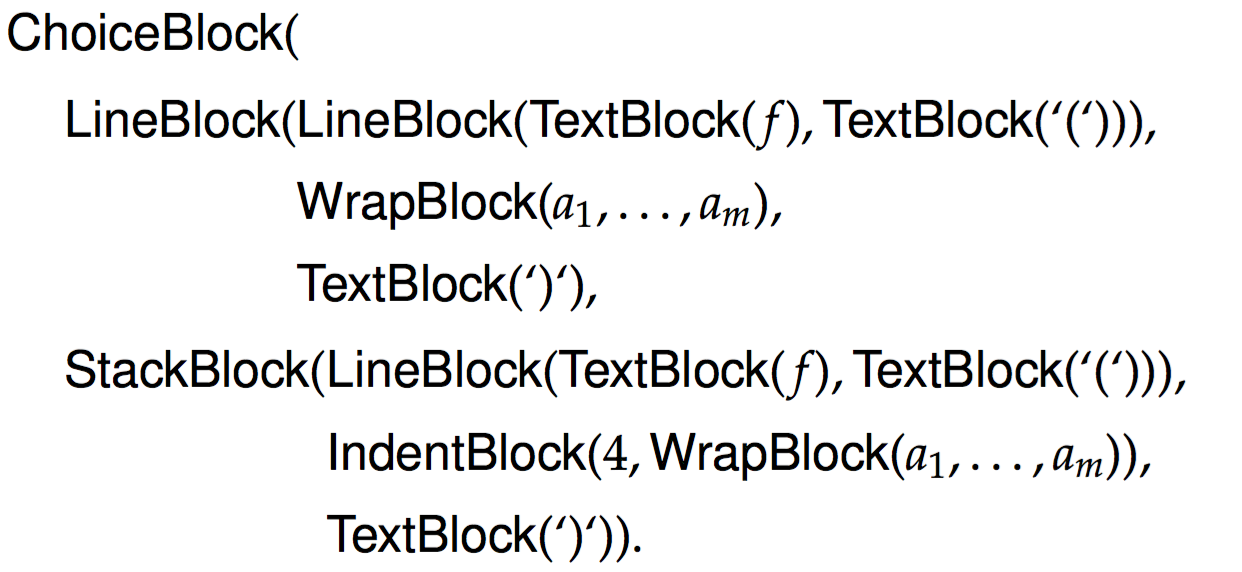
\includegraphics[width=0.8\textwidth]{img/block-rfmt.png}
        \end{center}
  \end{itemize}
\end{frame}

\begin{frame}{Line breaking: dynamic programming}
  \begin{minipage}{0.45\textwidth}
    \begin{itemize}
      \item Dynamic programming to find optimal line breaking
        \begin{itemize}
          \item (AST node, column) pairs are keys
          \item can extrapolate missing columns
        \end{itemize}
    \end{itemize}
  \end{minipage}
  \begin{minipage}{0.5\textwidth}
    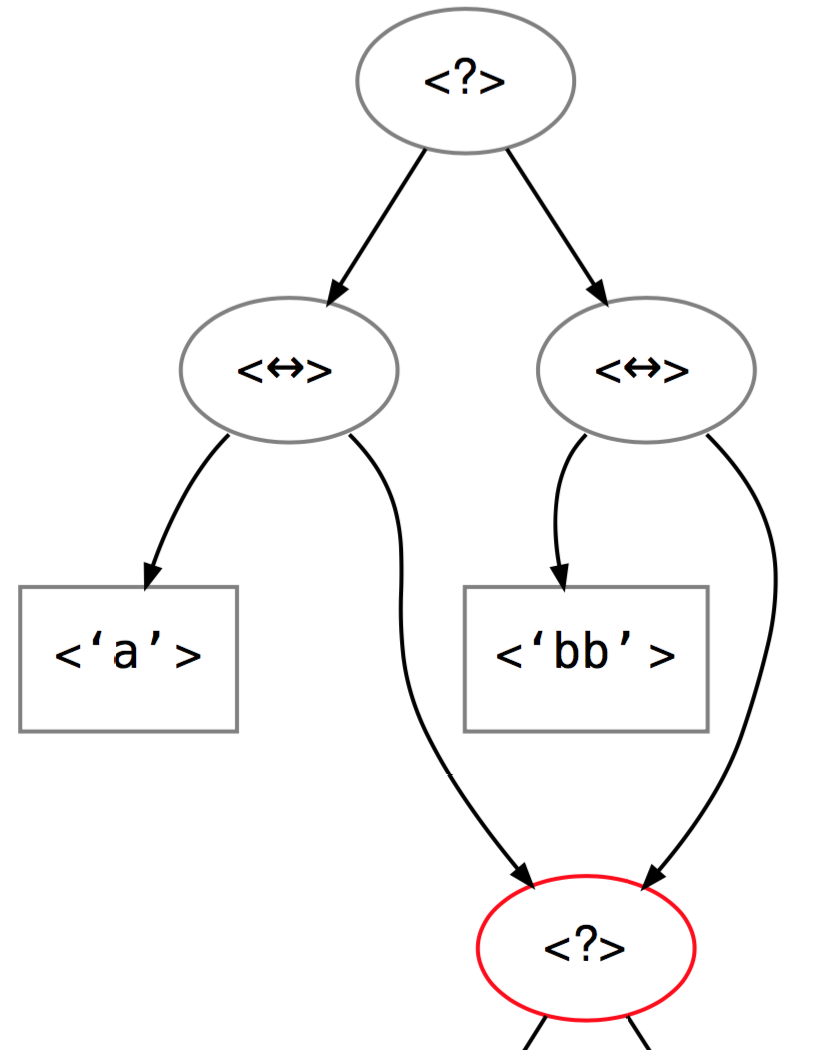
\includegraphics[width=0.9\textwidth]{img/dp-rfmt.png}
  \end{minipage}
\end{frame}
%%%%%%%%%%%%%%%%%%%%%%%%%%%%%%%%%%%%%%%%%%%%%%%%%%%%%%%%%%%%%%%
% 2. Scalafmt
%%%%%%%%%%%%%%%%%%%%%%%%%%%%%%%%%%%%%%%%%%%%%%%%%%%%%%%%%%%%%%%
\section{scalafmt} % (fold)
\label{sec:scalafmt}

\begin{frame}{Architecture}
  \begin{center}
    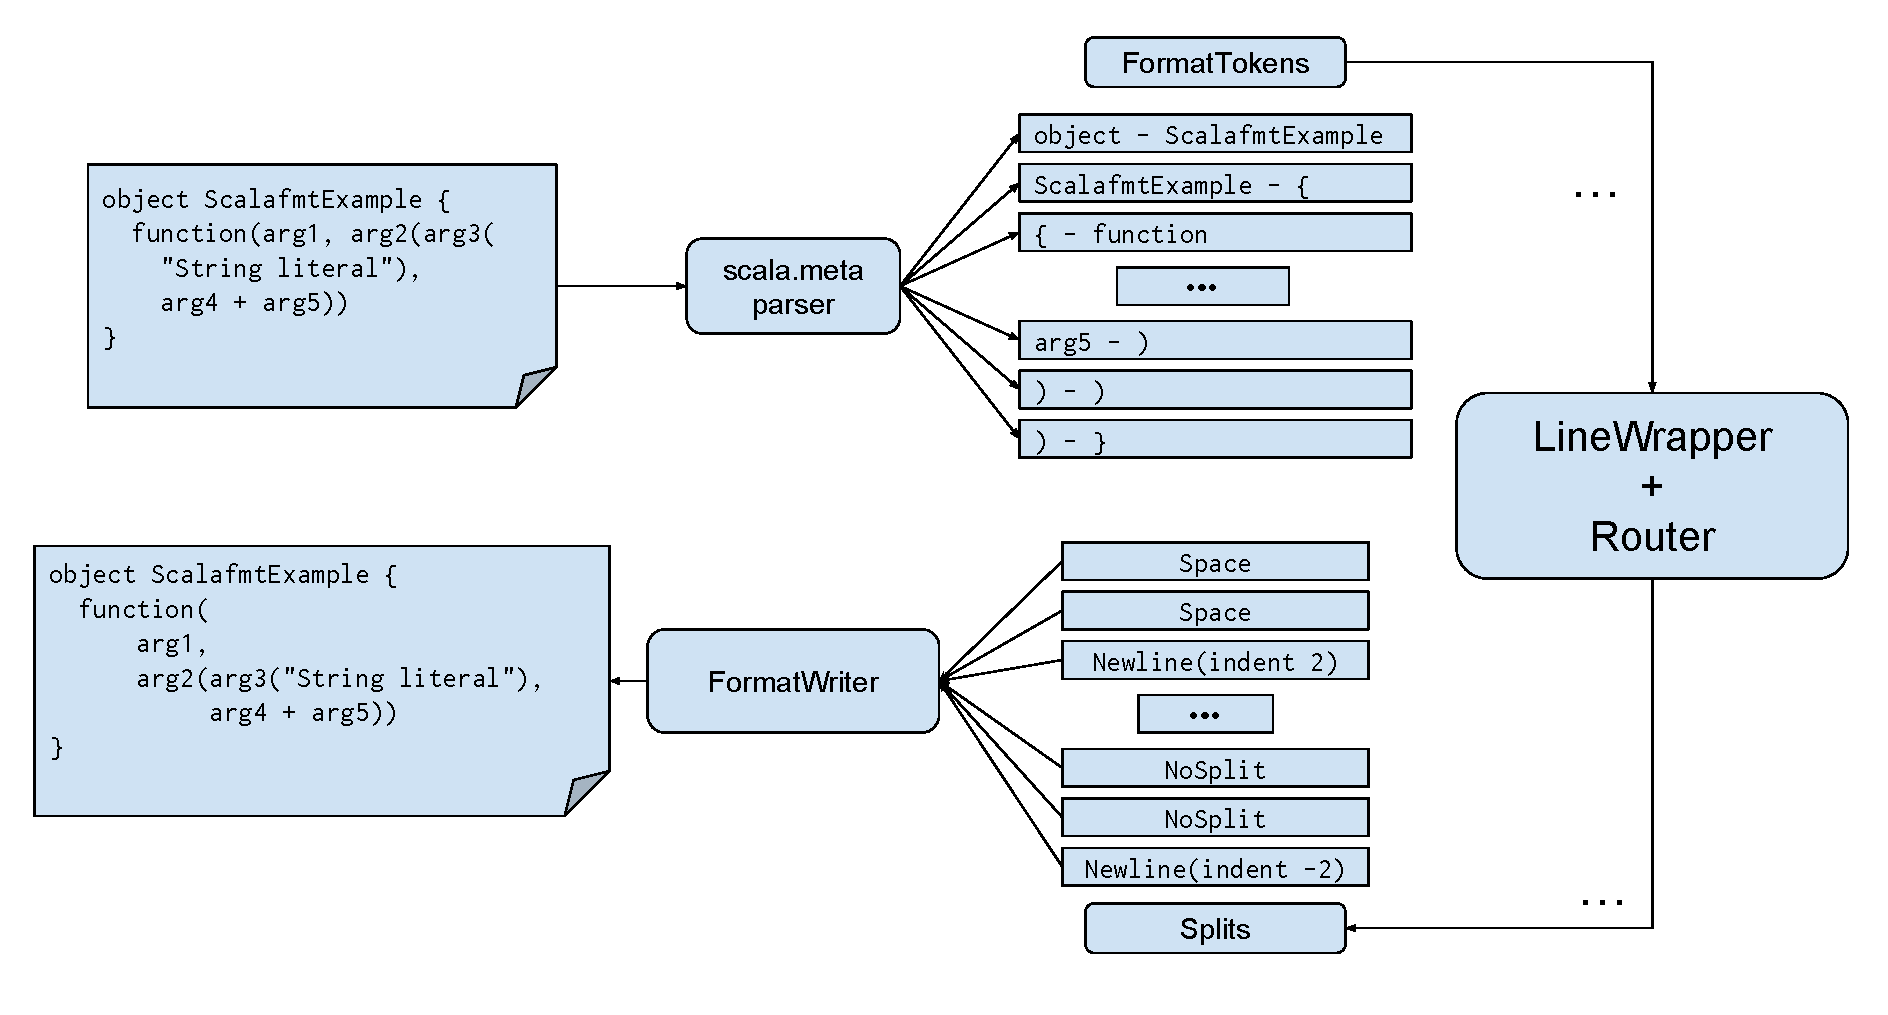
\includegraphics[width=0.9\textwidth]{img/architechture.pdf}
  \end{center}
\end{frame}


% \subsection{Data structures} % (fold)
%
% \begin{frame}{FormatToken}
%   \lstinputlisting{code/format_token.scala}
% \end{frame}
%
% \begin{frame}{Split}
%   
% \end{frame}
%
\subsection{Algorithms} % (fold)

\begin{frame}{LineWrapper + Router}
  \begin{center}
    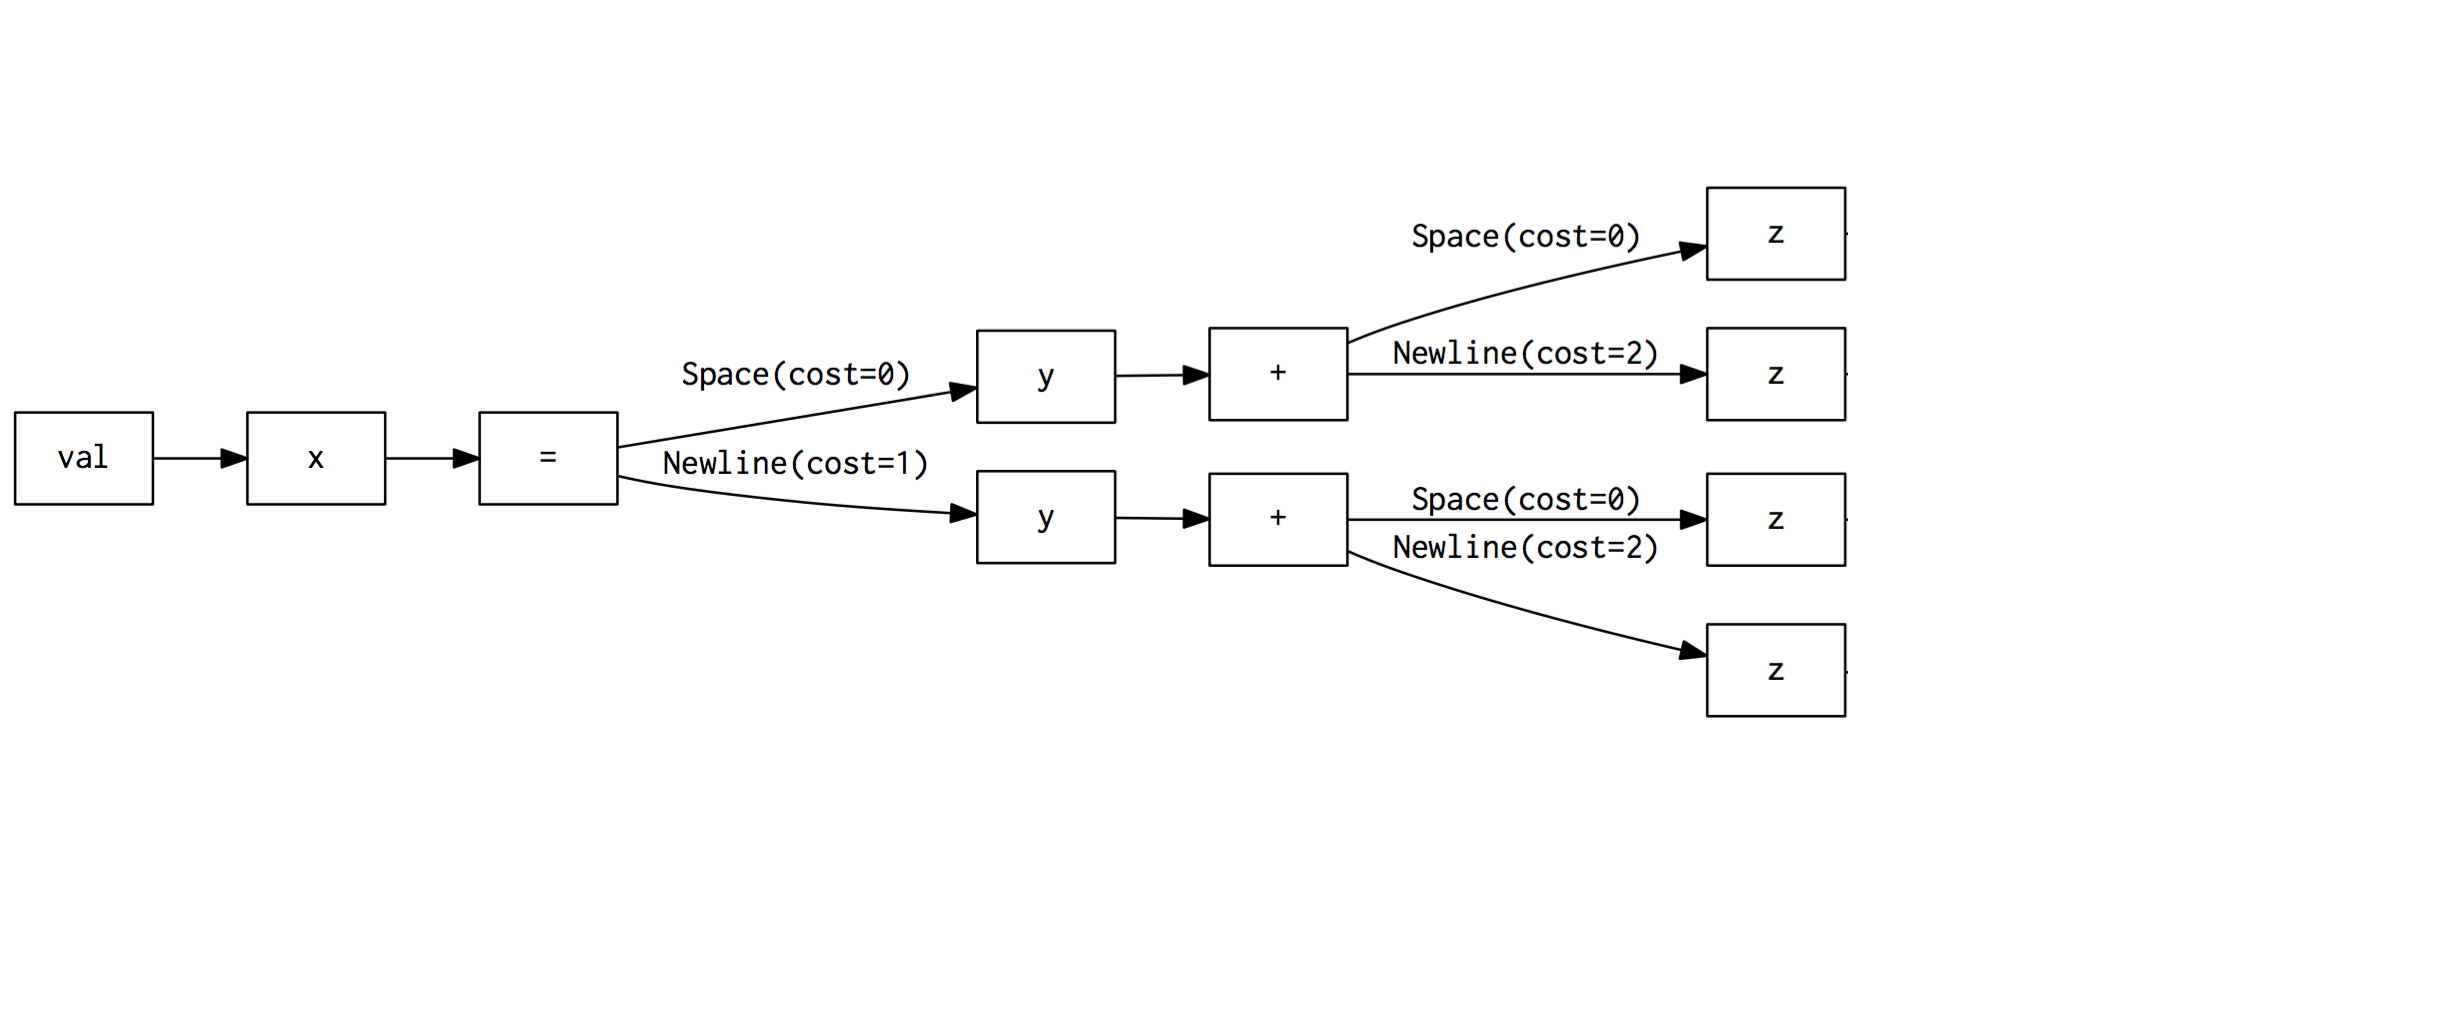
\includegraphics[width=\textwidth]{img/router1.png}
  \end{center}
\end{frame}

\begin{frame}{LineWrapper + Router}
  \begin{center}
    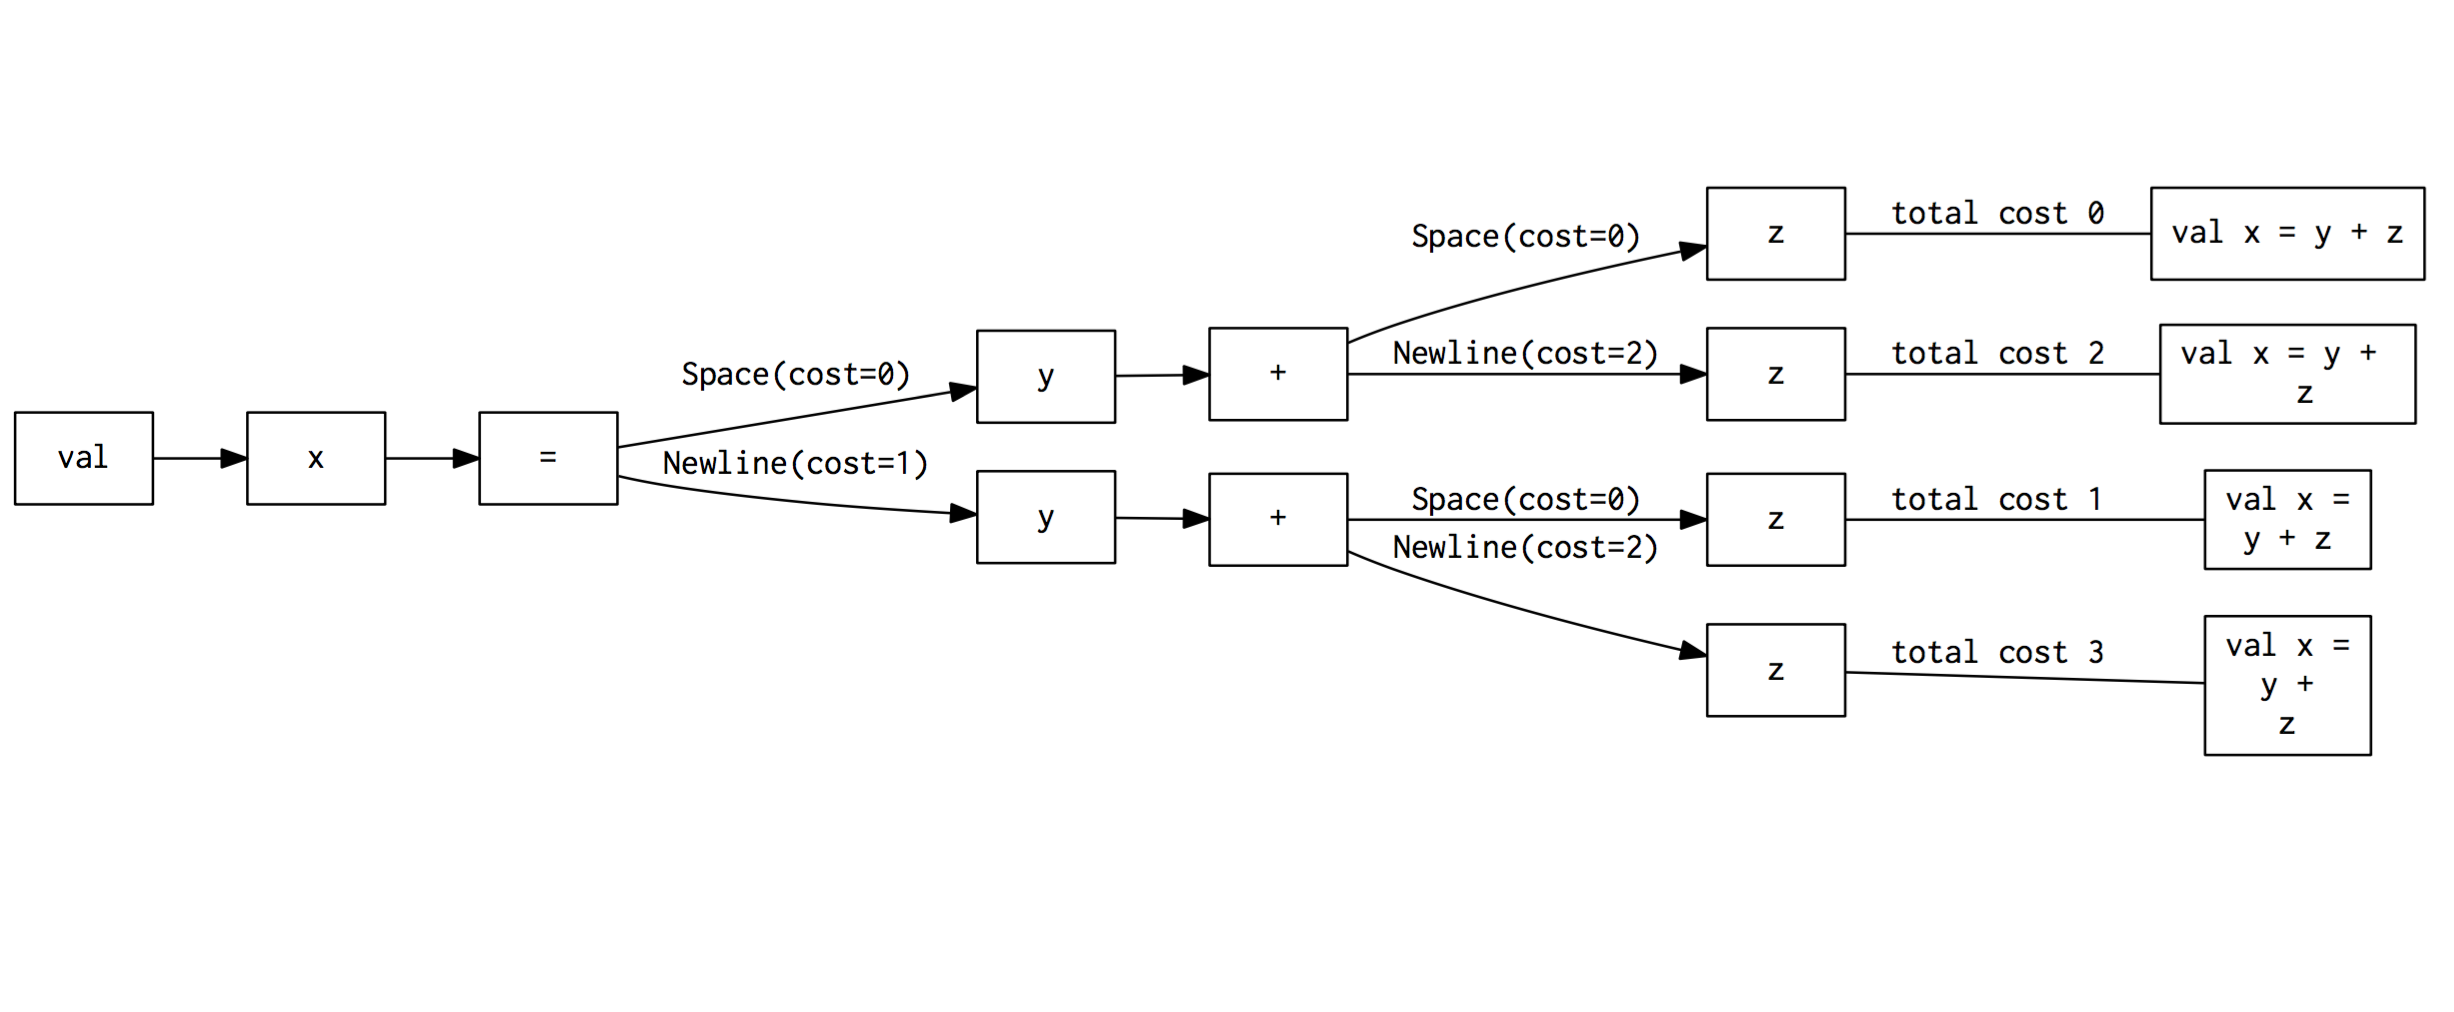
\includegraphics[width=\textwidth]{img/router2.png}
  \end{center}
\end{frame}

\begin{frame}{Router}
  \begin{itemize}
    \item One big pattern match ($\sim$ 1.100 LOC) on pairs of tokens
  \end{itemize}
  \lstinputlisting[basicstyle={\scriptsize\ttfamily}]{code/match.scala}
\end{frame}

\newcommand{\naive}{Na\"{\i}ve}

\begin{frame}{\naive{} best-first search}
  \begin{itemize}
    \item Small: $\sim$ 20 LOC
    \item Exponential running time for basic programs
  \end{itemize}
\end{frame}


\begin{frame}{Optimization 1: dequeueOnNewStatements}
  \lstinputlisting{code/dequeue.scala}
\end{frame}

\begin{frame}{Optimization 2: OptimalToken}
  \lstinputlisting{code/optimal.scala}
\end{frame}

\begin{frame}{Optimization 3: escapeInPathologicalCases}
  \begin{itemize}
    \item Give up, default behavior
    \item Best-effort, \texttt{--bestEffortInDeeplyNestedCode}
  \end{itemize}
  \lstinputlisting{code/pathological.scala}
\end{frame}

% \begin{frame}{Putting it all together}
%   \lstinputlisting{code/example-split.scala}
% \end{frame}

\begin{frame}{Vertical alignment}
  \begin{itemize}
    \item Implementation: 130 LOC imperative
    \item Running time: linear
    \item Configuration: \texttt{--alignTokens =>;Case,->;Infix,//;.*}
  \end{itemize}
  \lstinputlisting{code/align2.scala}
\end{frame}

\begin{frame}{Summary: algorithms}
  \begin{table}[H]
    \centering
    \label{}
    \begin{tabular}{ll}
      Component & Lines of code \\
      \hline \hline
      Router & 1.070 \\
      FormatWriter & 175 \\
      Best-first search & 369 \\
      Utilities and data structures & 1.547 \\
      \hline
      Total & 3.161
    \end{tabular}
  \end{table}
\end{frame}

\subsection{Testing}

\begin{frame}{}
  \begin{center}
    \Huge Testing?
  \end{center}
\end{frame}

\begin{frame}{Property 1: can format}
  \lstinputlisting{code/canformat.scala}
\end{frame}

\begin{frame}{Property 2: can format}
  \lstinputlisting{code/astintegrity.scala}
\end{frame}

\begin{frame}{Property 3: idempotent}
  \lstinputlisting{code/idempotent.scala}
\end{frame}

\subsection{Tooling} % (fold)

\begin{frame}{}
  \begin{center}
    \Huge Tooling
  \end{center}
\end{frame}

\begin{frame}{Heatmap}
  \begin{center}
    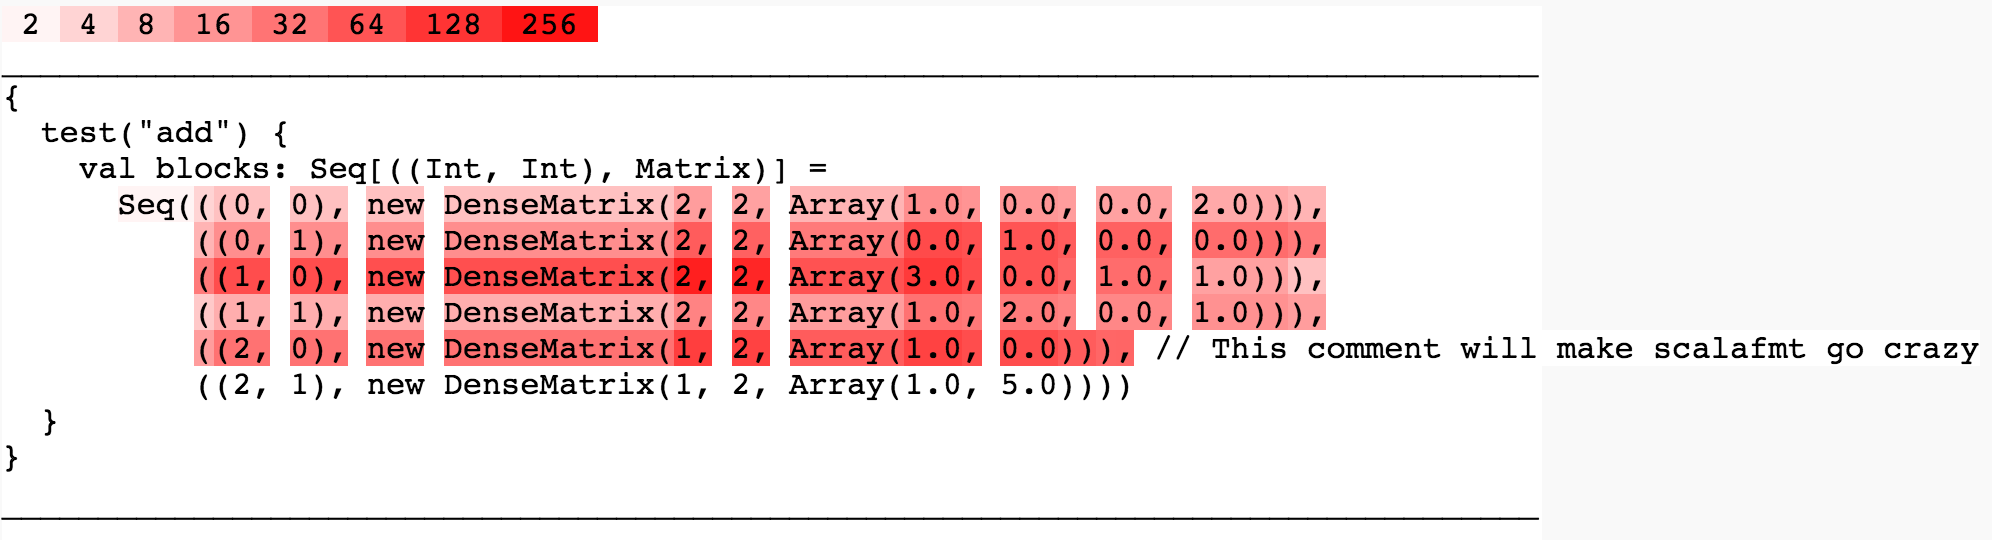
\includegraphics[width=0.9\textwidth]{img/heatmap.png}
  \end{center}
\end{frame}

\begin{frame}{Diff heatmap}
  \begin{center}
    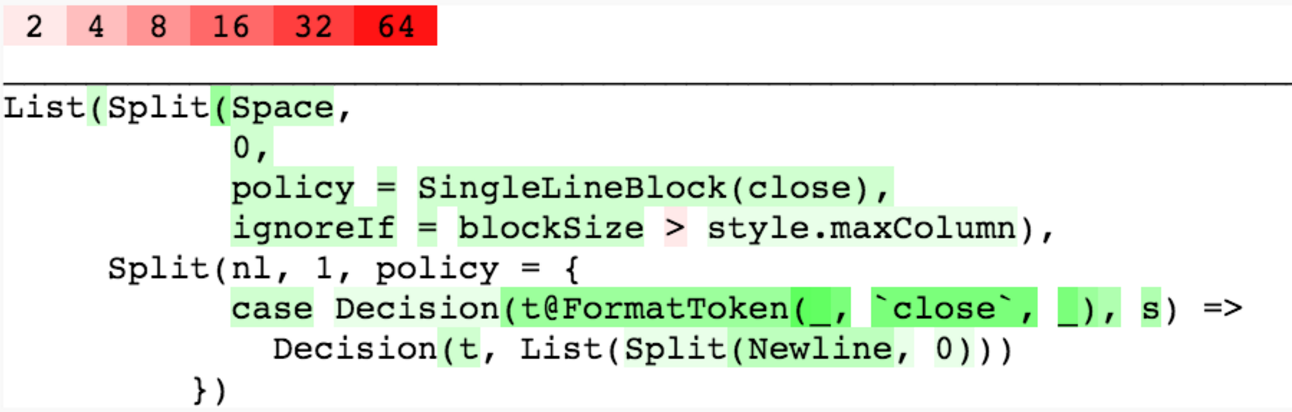
\includegraphics[width=0.9\textwidth]{img/heatmap2.png}
  \end{center}
\end{frame}


%%%%%%%%%%%%%%%%%%%%%%%%%%%%%%%%%%%%%%%%%%%%%%%%%%%%%%%%%%%%%%%
% 3. Conclusion
%%%%%%%%%%%%%%%%%%%%%%%%%%%%%%%%%%%%%%%%%%%%%%%%%%%%%%%%%%%%%%%
\section{Results} % (fold)
\label{sec:Results}

\subsection{Performance}


\begin{frame}{Macro benchmark}
  \begin{block}{Insight}
    How does scalafmt perform in a continuous integration setup?
  \end{block}
  \begin{block}{Task}
    Format Scala.js repo.
  \end{block}
\end{frame}

\begin{frame}{Macro benchmark}
  \begin{table}[H]
    \centering
    \begin{tabular}{lllll}
  Benchmark                &  Cores  &   Score  &   Error &  Units\\
  \hline
  \hline
  Parallel.scalafmt        &  4      &  14.616  &   0.632 &   s/op\\
  Parallel.scalariform     &  4      &   2.810  &   0.641 &   s/op\\
\hline
  Ratio &  & 5.20 &  & \\
  \\
  Synchronous.scalafmt     &  1      &  35.654  &   0.459 &   s/op\\
  Synchronous.scalariform  &  1      &   5.951  &   0.135 &   s/op\\
\hline
  Ratio &  & 5.99 &  & 
\end{tabular}

  \end{table}
\end{frame}

\begin{frame}{Micro benchmark}
  \begin{block}{Insight}
     How does scalafmt perform in an interactive software developer workflow?
  \end{block}
  \begin{block}{Task}
    Format single source file.
  \end{block}
\end{frame}

\begin{frame}{File sizes}
  \begin{table}[H]
    \centering
    \caption{Lines of code per source file. Collected from sample of $\sim$27.000 source files with total 3.2 million lines of code.}\label{tab:micro}
    \begin{tabular}{llllllll}
  25th & Median & Mean & 75th & 90th & 95th & 99th & Max\\
  \hline
  \hline
  16 & 46 & 106 & 113 & 248 & 400 & 945 & 11.723\\
  
\end{tabular}

  \end{table}
  \begin{itemize}
    \item Small: $\sim$ 50 LOC
    \item Medium: $\sim$ 300 LOC
    \item Large: $\sim$ 1.000 LOC
    \item Extra large: $\sim$ 4.500 LOC
  \end{itemize}
\end{frame}

\begin{frame}{Micro benchmark: results}
  \begin{table}[H]
    \centering
    \begin{tabular}{llll}
  Benchmark              &     Score &     Error &  Units\\
  \hline
  \hline
  Small.scalafmt         &     6.968 &    0.104 &  ms/op\\
  Small.scalariform      &     1.176 &    0.025 &  ms/op\\
  \hline
  Ratio            &   5.93   &  &    \\
  \\
  Medium.scalafmt        &    79.616 &    2.013 &  ms/op\\
  Medium.scalariform     &    15.934 &    0.441 &  ms/op\\
\hline
  Ratio            &   5.00   &  &
\end{tabular}

  \end{table}
\end{frame}

\begin{frame}{Micro benchmark: results}
  \begin{table}[H]
    \centering
    \begin{tabular}{llll}
  Benchmark              &     Score &     Error &  Units\\
  \hline
  \hline
  \\
  Large.scalafmt         &   355.819 &  17.385  &  ms/op\\
  Large.scalariform      &    39.324 &    3.395 &  ms/op\\
\hline
  Ratio            &   9.05   &  & \\
  \\
  ExtraLarge.scalafmt    &  1423.140 &  103.360 &  ms/op\\
  ExtraLarge.scalariform &   219.820 &   14.450 &  ms/op\\
\hline
  Ratio            &   6.50   &  &
\end{tabular}

  \end{table}
\end{frame}


\subsection{User adoption}

\begin{frame}{Installations}
  \begin{table}[]
    \centering
    \caption{Download numbers for scalafmt}
    \begin{tabular}{lll}
  Channel          & Version  &  Installations\\
  \hline
  \hline
  IntelliJ         & v0.2.5   &  847            \\
                   & All      &  3.273\\
  Maven            & v0.2.5   &  788            \\
                   & All      &  2.657          \\
  Github           & v0.2.5   &  102            \\
                   & All      &  929            \\
\hline
  Sum        & v0.2.5   &  1.737          \\
                   & All      &  6.859          
\end{tabular}
 
  \end{table}
\end{frame}

\begin{frame}{Installations}
  \begin{figure}[H]
    \centering
    
\includegraphics[angle=-90,width=0.5\textwidth]{tables/month.eps}
    \caption{Scalafmt installations by month by channel}
  \end{figure}
\end{frame}



\section{Conclusion} % (fold)
\label{sec:Conclusion}

\begin{frame}{Conclusions}
  \begin{table}
    \centering
    \begin{tabular}{ll}
      Maximum line length setting & X \\
      Opinionated settings        & X \\
      Vertical alignment          & X \\
      Performance                 & ?\footnote{Seems many users are OK with
                                               current performance}
    \end{tabular}
  \end{table}
\end{frame}

\begin{frame}{Verizon}
  \begin{quote}
    ``Verizon is now including scalafmt (with reformat on compile settings) in
    the default template for all new projects (which, in a sizable
    microservices shop, is a lot of projects)''

    \hfill --- Daniel Spiewak\footnote{Source: \url{https://gitter.im/olafurpg/scalafmt?at=5776b518cdab7a1f4fbefd31}}
  \end{quote}
\end{frame}


\begin{frame}[fragile]
  \frametitle{The End}
    \begin{center}
      \Huge
        Thank you!
    \end{center}
\end{frame}


\end{document}
